\dummypart{2}{Polynomials}
\myLesson{Factors, Roots, Solutions, Zeros, and \texorpdfstring{$x$}-intercepts}[10]

\begin{myObjectives}
    \myObjective{convert}{%
        between the following
        \begin{itemize}[nosep]
            \item the \gap{linear} \gap{factors} of $f(x)$
            \item the \gap{$x$-intercepts} of $f(x)$
            \item the \gap{zeros} of $f(x)$
            \item the \gap{roots} or \gap{solutions} of $f(x)=0$
        \end{itemize}
    }
\end{myObjectives}

\begin{myVocabulary}
    \myDefinition{$x$-intercepts}{%
        points where {a graph} \gap{crosses} the $x$-axis
    }
    \myDefinition{zeros of $f(x)$}{%
        $x$ values where {the function} is \gap{zero}
    }
    \myDefinition{roots, solutions}{$x$ values you get when you \gap{solve} $f(x)=0$ }
    \myDefinition{linear factor}{a factor of $f(x)$ that looks like \gap{$(x-a)$}} 
\end{myVocabulary}


\section{Introduction}

The key to solving absolute value 
\myEmph{equations} was to think about \gap{distance}.

\begin{tcolorbox}[width=4in, center, colback=white,]
    $|x| = 3$
    \tcblower
    \begin{center}
        \begin{tcolorbox}[center,colback=white,boxrule=0.5pt,]
            \small The distance of $x$ from the origin is \myEmph{equal to} $3$.
        \end{tcolorbox}
        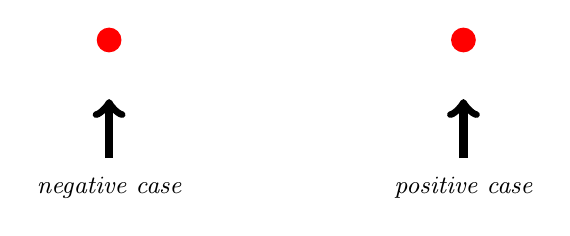
\begin{tikzpicture}[scale=0.75]
            \myDrawNumberlineCircle{0}{white}
            \whenTEACHER{
                % \draw [->,line width=3pt,red] (-3,-2) -- (-3,-1);
                \draw[red,line width=2.5pt,fill=red] (-3,0) circle (0.15 cm);
                %
                % \draw [->,line width=3pt,red] (3,-2) -- (3,-1);
                \draw[red,line width=2.5pt,fill=red] (3,0) circle (0.15 cm);
                }
                \draw[->, black, line width=3pt] (-3,-2) -- (-3,-1);
                \node[] at (-3,-2.5) {\itshape\small negative case};
                \draw[->, black, line width=3pt] (3,-2)  -- (3,-1);
                \node[] at (3,-2.5) {\itshape\small positive case};
                \myDrawNumberline{5}
        \end{tikzpicture}\\
        \whenSTUDENT{\vspace{3\onelineskip}}
        %
        \whenTEACHER{
            {
                $x = -3$
            }
            \hfil
            {
                $x = 3$
            }
        }
    \end{center}
\end{tcolorbox}

Similarly,
the key to solving absolute value
\myEmph{inequalities} is to think about \gap{distance}.


In the last lesson, we added rational expressions. 
We simplified expressions that looked like this.
\[
    \frac
    {(x-2)}
    {(x+3)}
    +
    \frac
    {3x}
    {(x+3)(x+5)}
\]
%
Today we will subtract like this:
\[
    \frac
    {(x-2)}
    {(x+3)}
    \bm{-}
    \frac
    {3x}
    {(x+3)(x+5)}
\]


\begin{tcolorbox}[center,colback=white,width=7in,]
    {\bfseries\itshape Subtraction} 
    is mostly the same as addition.
    The key idea is to combine the fractions 
    over a common \gap{denominator} (LCD).\par
    \vspace{1em}
    But for subtraction, 
    you need to remember to \gap{distribute} the negative.
    This is easy to forget!
\end{tcolorbox}

\begin{myConceptSteps}{To {\bfseries\itshape subtract} two rational expressions\dots}
    \myStep{common denominator}{
        If the fractions have \gap{different} denominators\dots
        \begin{itemize}[nosep]
            \item Factor the denominators.
            \item Find the \gap{LCD} of the two rational expressions.
            \item \gap{Multiply} the numerators and denominators 
            by factors needed to make their denominators equal to the \gap{LCD}.
        \end{itemize}
    }
    \myStep{subtract}{%
        Subtract the \gap{numerators}.
        \begin{itemize}[nosep]
            \item{\bfseries\itshape Do not} subtract the denominators.
            The denominator becomes the \gap{LCD}. 
        \end{itemize}
    }
    \myStep{simplify}{%
        Simplify the expression.
        \begin{itemize}[nosep]
            \item Remember to \gap{distribute} the negative. 
        \end{itemize}
    }
\end{myConceptSteps}


\myWideProblem
    {
        $
        \frac{2x}{x^2+2x-8}
        -
        \frac{1}{2}
        $
    }
    {6.5in}
\section{Polynomial Long Division}

\begin{myConcept}{~To divide polynomials by long division \dots}
    \begin{center}
        \begin{tabular}{m{0.5\textwidth}|p{0.45\textwidth}}
            & 
            {\Large $ \frac{2x^2  -1}{x-3} $}
            \rule{0in}{1\baselineskip}
            \\ \hline
            {\bfseries\itshape Step 1.}
            Write the dividend and divisor
            as a long division problem.
            Write the polynomials in {\bfseries\itshape descending order}.
            Fill in {\bfseries\itshape zeros} for missing terms. 
            & 
            \rule{0in}{2\baselineskip}
            \\ \hline
            {\bfseries\itshape Step 2.}
            Divide the {\bfseries\itshape leading term} in the dividend 
            by the {\bfseries\itshape leading term} in the divisor.
            Write this above the dividend.
            & 
            \rule{0in}{4\baselineskip}
            \\ \hline
            {\bfseries\itshape Step 3.}
            Multiply the divisor by this expression (distribute).
            Write the new terms {\bfseries\itshape lined up} under the dividend.
            & 
            \rule{0in}{4\baselineskip}
            \\ \hline
            {\bfseries\itshape Step 4.}
            {\bfseries\itshape Subtract} to form a new polynomial.
            & 
            \rule{0in}{7\baselineskip}
            \\ \hline
            {\bfseries\itshape Step 5.}
            {\bfseries\itshape Repeat} with the new polynomial.
            & 
            \rule{0in}{9\baselineskip}
            \\ \hline
            {\bfseries\itshape Step 6.}
            Stop when there is nothing left to bring down.
            The {\bfseries\itshape quotient} is the polynomial above the dividend.
            Write the {\bfseries\itshape remainder} as a fraction over the divisor.
            & 
            \\ 
        \end{tabular}
    \end{center}
\end{myConcept}

\myProblems[Divide these polynomials.]
    {
        $
            (3x^3 - 8x^2 - 13x + 9) 
            \div
            (3x+4)
        $
    }
    {
        \Large
        $\frac
            {2x^4 - 5x^2 - 2x - 11} 
            {x^2 - 4}
        $
    }
    {5in}

\section{Transformations Cheat Sheet}

\begin{tcolorbox}[center,colback=white,width=3.5in,valign=center,]
{
    \vspace{-0.9\onelineskip}
    \begin{equation*}
        f(x)=b^x \text{\quad\huge$\rightarrow$\quad} g(x) = \bm{a} \, b^{x - \bm{h}} + \bm{k}
    \end{equation*}
}
\end{tcolorbox}
\begin{myWarningBox}
    \begin{center}
        Remember that $\bm{h}$ is the \gap{opposite} 
        of what you see in the formula for $g(x)$.
    \end{center}
\end{myWarningBox}


{
\small 
\begin{tcbraster}[
    raster columns = 2,
    raster equal height,
    colback = white,
    % raster left skip = 0.75in, raster right skip = 0.75in, raster column skip = 0.75in,
    % raster before skip = 0.25in, raster after skip = 0.25in,
]
    \begin{tcolorbox}[
        title=Transformations, 
        coltitle=black, 
        colbacktitle=black!20, 
        fonttitle=\sffamily\bfseries\centering\large,
        boxrule=0.5pt,
        ]
        \centering
        \renewcommand{\arraystretch}{1.75}
        % {\small $|\bm{a}|, |\bm{h}|, |\bm{k}|$ \itshape mean \gap{ignore} the sign}
        \begin{tabular}[t]{|>{\raggedright}p{1in}|p{1.75in}|}
            \hline
            {\itshape vertical} {\bfseries\itshape reflection} 
            & if $\bm{a}$ is \gap{negative}\\ 
            % & \\
            % & \\
            \noalign{\hrule height 0.25pt}
            {\itshape vertical} {\bfseries\itshape stretch} by $|\bm{a}|$
            &  if $|\bm{a}|$  is \gap{$> 1$} \\ 
            % & \\
            % & \\
            \noalign{\hrule height 0.25pt}
            {\itshape vertical} {\bfseries\itshape compression} by $|\bm{a}|$
            &  if $|\bm{a}|$ is \gap{$< 1$} \\ 
            % & \\
            % & \\
            \noalign{\hrule height 1.5pt}
            {\itshape horizontal shift} {\bfseries\itshape right} by $|\bm{h}|$
            &  if $\bm{h}$  is \gap{positive}\\ 
            % & \\
            % & \\
            \noalign{\hrule height 0.25pt}
            {\itshape horizontal shift} {\bfseries\itshape left} by $|\bm{h}|$
            &  if $\bm{h}$  is \gap{negative}\\ 
            % & \\
            % & \\
            \noalign{\hrule height 1.5pt}
            {\itshape vertical shift} {\bfseries\itshape up} by $|\bm{k}|$
            &  if $\bm{k}$  is \gap{positive}\\ 
            % & \\
            % & \\
            \noalign{\hrule height 0.25pt}
            {\itshape vertical shift} {\bfseries\itshape down} by $|\bm{k}|$
            &  if $\bm{k}$  is \gap{negative}\\ 
            % & \\
            % & \\
            \hline
        \end{tabular}
    \end{tcolorbox}
    \begin{tcolorbox}[
        title=Attributes, 
        coltitle=black, 
        colbacktitle=black!20, 
        fonttitle=\sffamily\bfseries\centering\large,
        boxrule=0.5pt,
        ]
        \centering
        \renewcommand{\arraystretch}{1.145}
        \begin{tabular}[t]{|>{\raggedright}p{0.75in}|p{2in}|}
            \hline
            {\bfseries\itshape G or D?} & if {$b>1$}: \whenTEACHER{growth}\\
            {}                                  & if {$0<b<1$}: \whenTEACHER{decay}\\
            % {} & \\
            \noalign{\hrule height 1.5pt}
            \hline
            {\bfseries\itshape horiz. asymp.} & \whenTEACHER{$y=k$}\\
            & \\
            \noalign{\hrule height 1.5pt}
            {\bfseries\itshape domain} & \whenTEACHER{all real numbers}\\
            % & \\
            \noalign{\hrule height 1.5pt}
            {\bfseries\itshape range} & if {$\bm{a}>0$}:\\
            {}                        & \whenTEACHER{$y > k$}\\
            % {}                        & \\
            {} & if {$\bm{a}<0$} (reflected):\\
            {} & \whenTEACHER{$y < k$}\\
            % {} & \\
            \noalign{\hrule height 1.5pt}
            {\itshape\bfseries end beh.} & if {$\bm{a}>0$}:  \\
            & \quad L: \whenTEACHER{as x{$\rightarrow-\infty$}, y{$\rightarrow 0$}}\\
            & \quad R: \whenTEACHER{as x{$\rightarrow+\infty$}, y{$\rightarrow+\infty$}}\\
            % & \\
            &  if {$\bm{a}<0$} (reflected): \\
            & \quad L: \whenTEACHER{as x{$\rightarrow-\infty$}, y{$\rightarrow 0$}}\\
            & \quad R: \whenTEACHER{as x{$\rightarrow+\infty$}, y{$\rightarrow-\infty$}}\\
            % {} & \\
            \hline
        \end{tabular}
    \end{tcolorbox}
\end{tcbraster}

}
\newpage
\section{Evaluating Absolute Value Functions}

\begin{tcolorbox}[center,width=6.5in,colback=white,]
    To evaluate a \gap{function} with absolute values, 
    you just \gap{evaluate} the expression for the function 
    at the input value.
\end{tcolorbox}


\myProblems[Evaluate these functions at the given input value.]
{ 
    $
        f(x) =
        |2x|
    $
    \qquad
    Find $f(6)$.
}
{
    $
        g(x) =
        3|-5x|
    $
    \qquad
    Find $g(30)$.
}
{8\onelineskip}

\myProblems
{
    $
        t(z) =
        |z - 8|
    $
    \qquad
    Find $t(2)$.
}
{
    $
        s(w) =
        1 - 2\left|w + 3\right|
    $
    \qquad
    Find $s(-5)$.
}
{8\onelineskip}


\myProblems[Find the values of $a$, $h$, $k$ in the following transformed reciprocal functions.]
{
    $g(x) = \frac{1}{x-2} + 3$
}
{
    $g(x) = \frac{5}{x+7} - 11$
}
{1.25in}

\myProblems
{
    $g(x) = \frac{-8}{x+7} + 9$
}
{
    $g(x) = \frac{-1}{x+7} - 1$
}
{1.25in}

\myProblems
{
    $g(x) = \frac{2}{4(x+5)} $
}
{
    $g(x) = -\frac{5}{3x} - 3 $
}
{1.25in}

